\documentclass[sokoban_generation_thesis.tex]{subfiles}

Metoda PDB \cite{heur_pdb} jest wprowadzona w~oparciu o~teorię problemu przeszukiwań przestrzeni stanu (ang.~\textit{state-space search problem}) oraz baz danych wzorców (ang.~\textit{pattern databases}). 

\subsection{Problem przeszukiwań przestrzeni} \label{subs:problem_przesz_przes}
Problemem przeszukiwań przestrzeni stanu nazywa się krotkę opisaną w~równaniu \ref{eq:sssproblem}. Składowe problemu to~kolejno zbiór stanów~$S$, stan początkowy~$s_0$, zbiór stanów docelowych~$S^*$ oraz zbiór akcji~$A$. Stan definiuje się jako pełne przypisanie wartości wszystkim zmiennym $v \in V$, przy zachowaniu dziedzin $D_v$. Rozwiązaniem problemu przeszukiwań przestrzeni jest ścieżka rozwiązująca (ang.~\textit{solution path}) -- skończony ciąg akcji, po~wykonaniu których ze~stanu~$s_0$ otrzyma się stan ze~zbioru~$S^*$. 

\begin{equation} \label{eq:sssproblem}
\mathcal{P} = <S, s_0, S^*, A>
\end{equation}

Opisywany problem różni się od~innych problemów przeszukiwania tym, że~przestrzeń stanów jest niejawna (ang.~\textit{implicit}). W~prezentowanym rozwiązaniu, graf przestrzeni stanów jest zbyt duży, aby można go~było wygenerować i~przechowywać w~pamięci. Zamiast tego, jedynie interesujące węzły są~generowane i~robione jest to~na~bieżąco -- w~trakcie ich eksploracji. Stanami w~metodzie PDB są~przypisania lokalizacji $k$ pudeł i~gracza, a~więc składają się z~$k+1$ zmiennych. Dziedziną każdej zmiennej są~puste pola. W~związku z~tym, liczba możliwych stanów opisana jest wzorem $(n-k)\binom{n-k-1}{k}$, gdzie $n$ to~liczba wolnych pól. Przykładowo, dla planszy małych rozmiarów przedstawionej na~rys.~\ref{rys:pdb_example} istnieje aż~$595\,980$ możliwych stanów (wierzchołków grafu).

\begin{figure}[h]
	\centering
	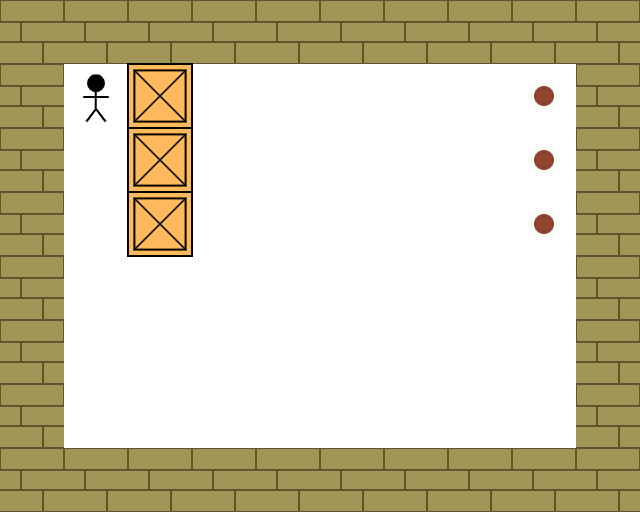
\includegraphics[width=0.3\textwidth]{board_pdb_example.png}
	\caption{Przykładowa plansza o~rozmiarze 8 x~10}
	\label{rys:pdb_example}
\end{figure}

Autorzy definiują ponadto problem wygenerowania początkowego stanu (ang.~\textit{initial state generation task}) $\mathcal{P}_{-s_0}$ \cite{heur_pdb}, opisany krotką w~równaniu \ref{eq:isgtask}. Jest on~równoważny problemowi przeszukiwań przestrzeni ze~stanem początkowym $s_0$, jednak celem nie jest wyznaczenie ścieżki, a~wskazanie stanu $s\in S$, dla którego problem $\mathcal{P}_{-s_0}$ z~$s$ jako stanem początkowym, jest rozwiązywalny.

\begin{equation} \label{eq:isgtask}
\mathcal{P}_{-s_0} = <S, S^*, A>
\end{equation}

W celu rozwiązania problemu opisanego w~niniejszym punkcie, stosuje się heurystykę bazy danych wzorców (ang.~\textit{pattern database heuristic}), wprowadzoną przez Josepha Culbersona oraz Jonathana Schaeffera \cite{pdb_original}. Idea tej heurystyki oparta jest na~zignorowaniu części problemu (podzbioru zmiennych $V$) i~wyznaczeniu dolnego ograniczenia długości ścieżki optymalnej dla pozostałych zmiennych. Pozostałe zmienne, dla których wyznaczane jest ograniczenie, nazywa się wzorcem. Jako lepsze ograniczenie stosuje się sumę wartości heurystyk dla rozłącznych wzorców, które pokrywają zbiór wszystkich zmiennych \cite{pdb_additive} -- wtedy mówi się o~bazie danych wzorców. Przykłady wykorzystania tej heurystyki w~metodzie PDB zostały opisane w~p.~\ref{subs:pdb_method_description}.

\subsection{Opis metody} \label{subs:pdb_method_description}
Metoda PDB rozpoczyna pracę w~oparciu o~rozwiązaną planszę \textit{Sokoban}. Plansza podawana na~wejściu algorytmu musi zawierać jedynie pudła na~polach docelowych oraz gracza, tak jak plansza na~rys.~\ref{rys:board_pdb_start}. Zadaniem metody jest wyznaczenie miejsc pudeł oraz zmodyfikowanie pozycji gracza tak, by~plansza była maksymalnie skomplikowana. Żeby nie musieć samodzielnie wyznaczać plansz początkowych, można korzystać z~wytworzonych przez ludzi plansz, odpowiednio je~modyfikując, co~zobrazowano na~rys.~\ref{rys:board_pdb_transform}.

\begin{figure}[h!]
	\centering
	\begin{subfigure}[b]{0.4\textwidth}
		\centering
		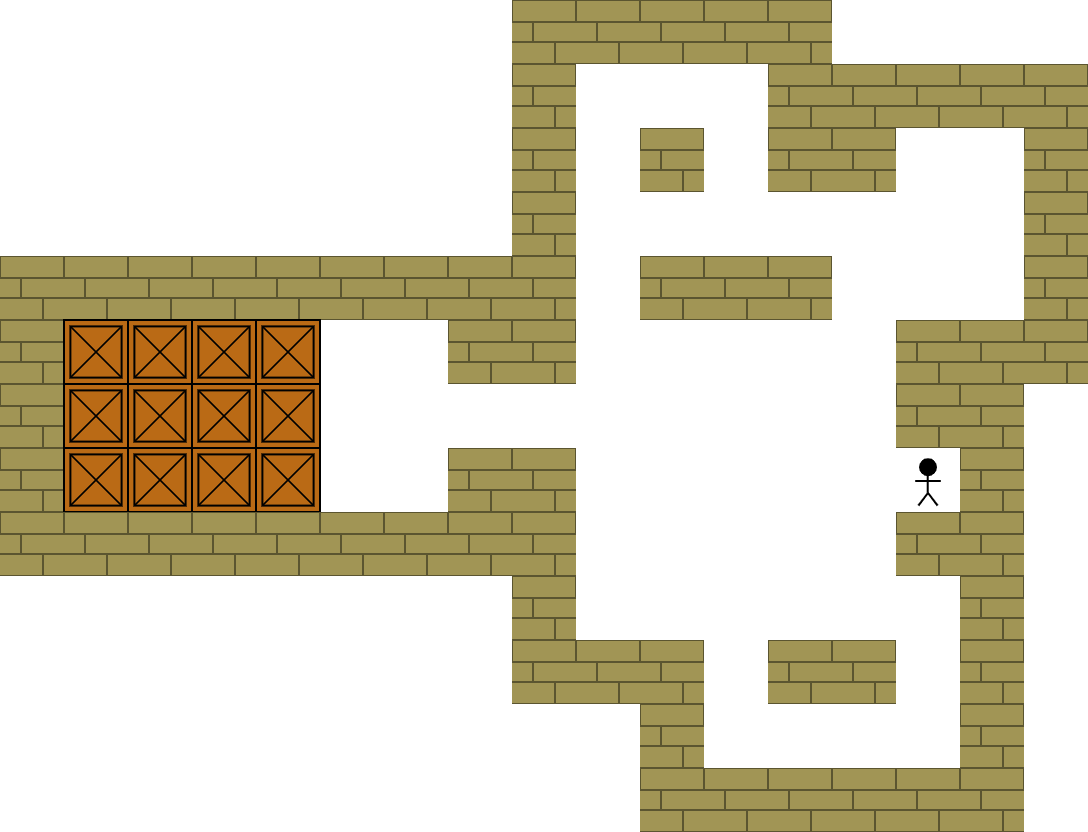
\includegraphics[width=\textwidth]{board_pdb_start}
		\caption{Plansza początkowa} \label{rys:board_pdb_start}
	\end{subfigure}
	\hspace{0.04\textwidth}
	\begin{subfigure}[b]{0.4\textwidth}
		\centering
		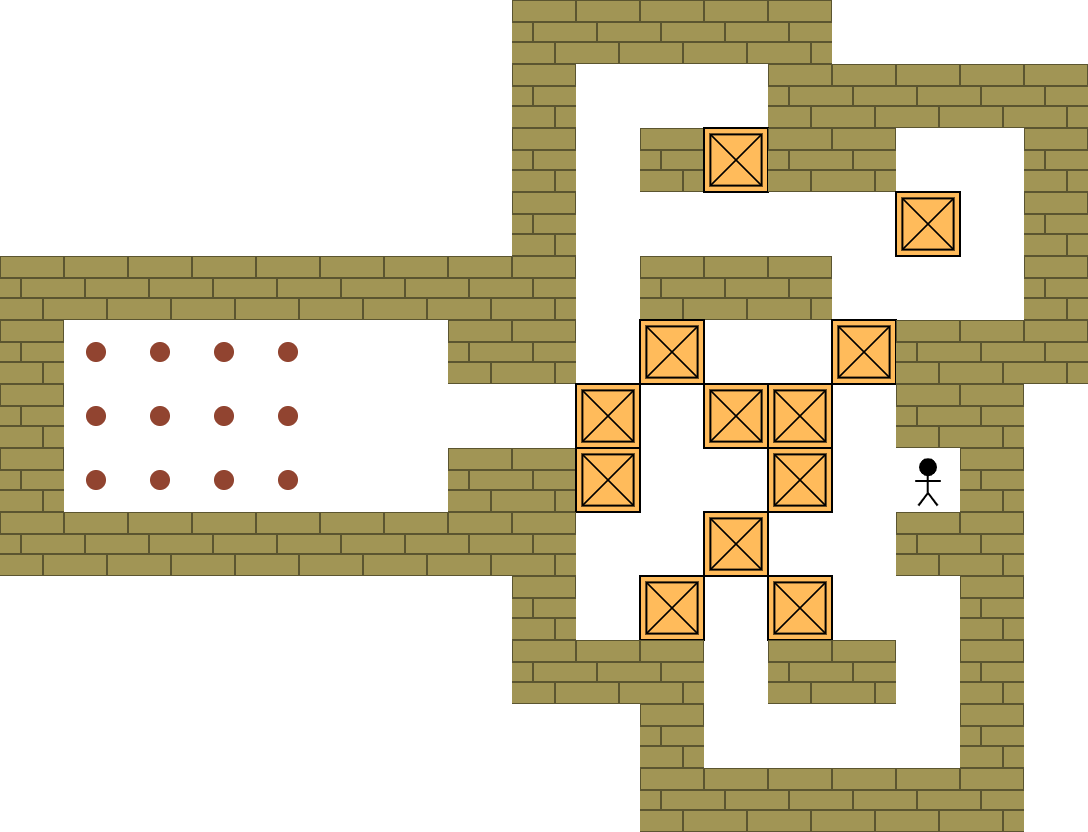
\includegraphics[width=\textwidth]{board_pdb_start_original}
		\caption{Plansza oryginalna}
	\end{subfigure}
	\caption{Plansza początkowa dla metody PDB wraz jej oryginalnym odpowiednikiem}
	\label{rys:board_pdb_transform}
\end{figure}

Algorytm $\beta$ \cite{heur_pdb}, wykorzystywany w~metodzie PDB, rozwiązuje problem przypisania miejsc pudeł i~gracza w~oparciu o~podejście zachłanne. W~tym celu wykorzystywane jest przeszukiwanie grafu, które priorytetyzuje węzły (ang.~\textit{best-first search}) zgodnie z~zadaną sekwencją $[\cdot]$. Graf stanów jest przeszukiwany wstecz, od~wierzchołka reprezentującego rozwiązaną planszę, co~gwarantuje istnienie ścieżki docelowej. Autorzy metody PDB podkreślają, że~przeszukiwanie grafu od~wierzchołka początkowego $s_p$ wymagałoby zapewnienia o~istnieniu ścieżki docelowej rozpoczynającej się w~$s_p$, co~jest wymagające obliczeniowo \cite{sokoban_pspace}.

Sekwencja $[\cdot]$ złożona jest z~wyselekcjonowanych wartości heurystyk wartościujących dany stan. Rodzaje wykorzystywanych heurystyk zostały wymienione poniżej. Autorzy metody wykorzystują różne konfiguracje sekwencji $[\cdot]$, co~zostało opisane dokładniej w~podrozdz.~\ref{subs:exp_pdb}.

\begin{itemize}
	\item $h^{PDB_k}$ - heurystyka bazy danych wzorców rozmiaru $k$.
	\item $w(h)$ - funkcja nowości.
	\item $kC$ - liczba konfliktów rzędu $k$.
\end{itemize}

$h^{PDB_k}$ to~heurystyka bazy danych wzorców rozmiaru $k$. W~przełożeniu na~problem generowania plansz \textit{Sokoban}, wartością heurystyki dla danego pudła (wzorca rozmiaru $1$) jest minimalna długość ścieżki, po~wykonaniu której pudło znajdzie się na~dowolnym polu docelowym. Przykładowo, plansza z~rys.~\ref{rys:board_pdb_heurexample} wymaga co~najmniej $16$ ruchów, by~ją~rozwiązać. Dla wzorców rozmiaru $1$, wartość heurystyki wynosi $1+2+2=5$, ponieważ górne pudło wymaga ścieżki złożonej z~jednego ruchu, a~dwa niższe -- z~dwóch ruchów (pozycja gracza jest nieistotna). Z~kolei heurystyka dla wzorców rozmiaru $2$ musi podzielić pudła na~zbiór dwu- oraz jednoelementowy. Jeśli wzorcem dwuelementowym będą dwa niższe pudła, to~minimalna liczba ruchów dla tego podproblemu wynosi $2+5=7$, ponieważ po~przepchnięciu jednego z~nich gracz musi się cofnąć i~przepchnąć drugie pudło. Finalnie, $h^{PDB_2}$ wynosi $1+(2+5)=8$. Podsumowując, $h^{PDB}$ stara się przybliżyć minimalną liczbę ruchów do~rozwiązania planszy. Warto zaznaczyć, że~współczynnik korelacji między długością optymalnej ścieżki a~czasem potrzebnym do~rozwiązania planszy \textit{Sokoban} w~teście rang Spearmana wynosi~$0.47$~\cite{sok_metrics2}.

\begin{figure}[h]
	\centering
	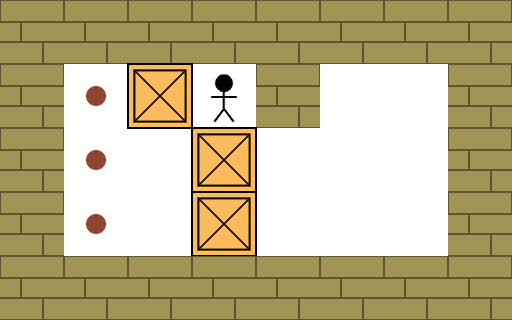
\includegraphics[width=0.25\textwidth]{board_pdb_heurexample}
	\caption{Przykładowa plansza}
	\label{rys:board_pdb_heurexample}
\end{figure}


Algorytm korzysta również z~funkcji nowości $w(h)$ (ang.~\textit{novelty function}) \cite{pdb_novelty}, która zwraca najwyższe wartości dla stanów, w~których zmienne przyjmują nieużywane wcześniej wartości. Implementacja $w(h)$ przechowuje licznik przypisań dla każdej zmiennej i~nagradza plansze, w~których pudło lub gracz trafiają na~dotychczas nieużyte lokacje.

Trzecim rodzajem używanych heurystyk jest liczba konfliktów rzędu $k$, która jest równa różnicy wartości heurystyki bazy danych dla wzorca rozmiaru $k$ i~$k-1$, przyjmując jedynie wartości nieujemne, jak w~wyrażeniu (\ref{eq:pdb_conflicts}). Dla planszy z~rys.~\ref{rys:board_pdb_heurexample} jest zatem $8-5=3$ konfliktów rzędu $2$. Istotnie, liczba ruchów gracza wymagana do~wycofania się celem przepchnięcia drugiego pudła to~$3$, co~autorzy metody nazywają ruchami nieintuicyjnymi (ang.~\textit{counterintuitive moves}). Warto zaznaczyć, że~współczynnik korelacji między tak wyznaczanymi ruchami nieintuicyjnymi a~czasem potrzebnym do~rozwiązania planszy \textit{Sokoban} w~teście rang Spearmana wyniósł~$0.69$~\cite{sok_metrics2}.

\begin{equation}\label{eq:pdb_conflicts}
	kC(s) = \max\left(h^{PDB_k}(s) - h^{PDB_{k-1}}(s);\,\, 0\right)  
\end{equation}

